% Gemini theme
% https://github.com/anishathalye/gemini

\documentclass[final]{beamer}

% ====================
% Packages
% ====================

\usepackage[T1]{fontenc}
\usepackage{lmodern}
\usepackage[size=custom,width=120,height=72,scale=1.0]{beamerposter}
\usetheme{gemini}
\usecolortheme{gemini}
\usepackage{graphicx}
\usepackage{booktabs}
\usepackage{tikz}
\usepackage{amssymb}
\usepackage{amsmath}
\usepackage{pgfplots}

% ====================
% Lengths
% ====================

% If you have N columns, choose \sepwidth and \colwidth such that
% (N+1)*\sepwidth + N*\colwidth = \paperwidth
\newlength{\sepwidth}
\newlength{\colwidth}
\setlength{\sepwidth}{0.025\paperwidth}
\setlength{\colwidth}{0.3\paperwidth}

\newcommand{\separatorcolumn}{\begin{column}{\sepwidth}\end{column}}

% ====================
% Title
% ====================

\title{Panviral Pepseq: A Highly Multiplexed Serological Diagnostic}

\author{Zane Fink\inst{1} \and Jason Ladner\inst{1}}

\institute[shortinst]{\inst{1} The Pathogen and Microbiome Institute at Northern Arizona University}

% ====================
% Body
% ====================

\begin{document}

\begin{frame}[t]
\begin{columns}[t]
\separatorcolumn

\begin{column}{\colwidth}

  \begin{block}{Abstract}

Viruses represent a diverse and ubiquitous challenge to the immune system, and a record of these encounters is preserved within our antibody responses. 
Understanding the diverse antiviral immune response has important implications for both epidemiology and immunology, 
but our capacity for characterizing this response has been historically limited due to the low throughput nature of the available assays. 
To circumvent these limitations, we are developing a high-throughput approach for serological characterization that begins with a custom set of oligonucleotides (oligos),
which are ultimately linked to the peptides they encode, in order to allow for direct interaction with serum antibodies.
To aid in the design of these oligos, we have developed algorithms to optimize coverage of a given set of viral proteins using fewer oligos than current algorithms.
By treating the design of these libraries as an instance of the weighted set cover problem, 
we can iteratively select the oligos that best represent the potential epitopes within a given reference set. 
Using these algorithms, we were able to cover an equal amount of peptide diversity with $20\%$ fewer oligos. 
By increasing the efficiency of design algorithms, we are able to cover more viral diversity within a single assay, 
greatly increasing the sensitivity of a single assay.

\end{block}


\begin{alertblock}{Objectives}
  \begin{itemize}
  \item \textbf{Design} an oligo library for Ab-PepSeq that broadly
    covers viruses that infect humans/mammals.
  \item \textbf{Create} algorithms for the efficient coverage of
    \emph{linear epitopes} (i.e., in as few oligos as possible).
  \item \textbf{Implement} these algorithms in an open source
    easy-to-use software package that is freely available for public use.
  \end{itemize}
\end{alertblock}
  % \begin{block}{Hypothesis}
  %   \begin{itemize}
  %   \item By treating the design of an oligonucleotide library as an instance
  %         of the weighted set cover problem, we can cover a grater range of epitope diversity
  %         in a smaller set of designed oligos.
  %   \end{itemize}

  % \end{block}
  \begin{block}{Background: What is PepSeq?}
    \begin{figure}
      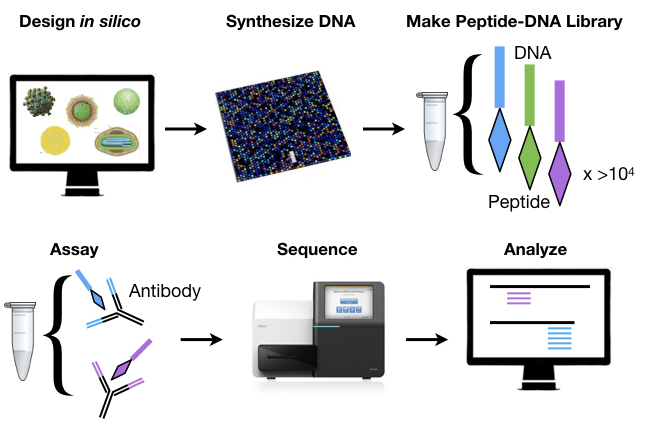
\includegraphics[width=0.6\colwidth]{figures/Overview.jpeg}
      \label{fig:library}
    \end{figure}
    \begin{itemize}
    \item Synthesize $100,000$s of DNA oligos that represent a diverse set of viral proteins.
    \item Serum antibodies used to enrich for recognized peptides
    \item Next-Generation Sequencing used for bulk characterization of enriched peptides.
    \item In this work we focus on the first step: \emph{Design in Silico}.

    \end{itemize}
  \end{block}
\end{column}

\separatorcolumn

\begin{column}{\colwidth}

  \begin{block}{Large Datasets Need to Be Clustered to Ensure Reasonable Runtime}
    \begin{figure}
      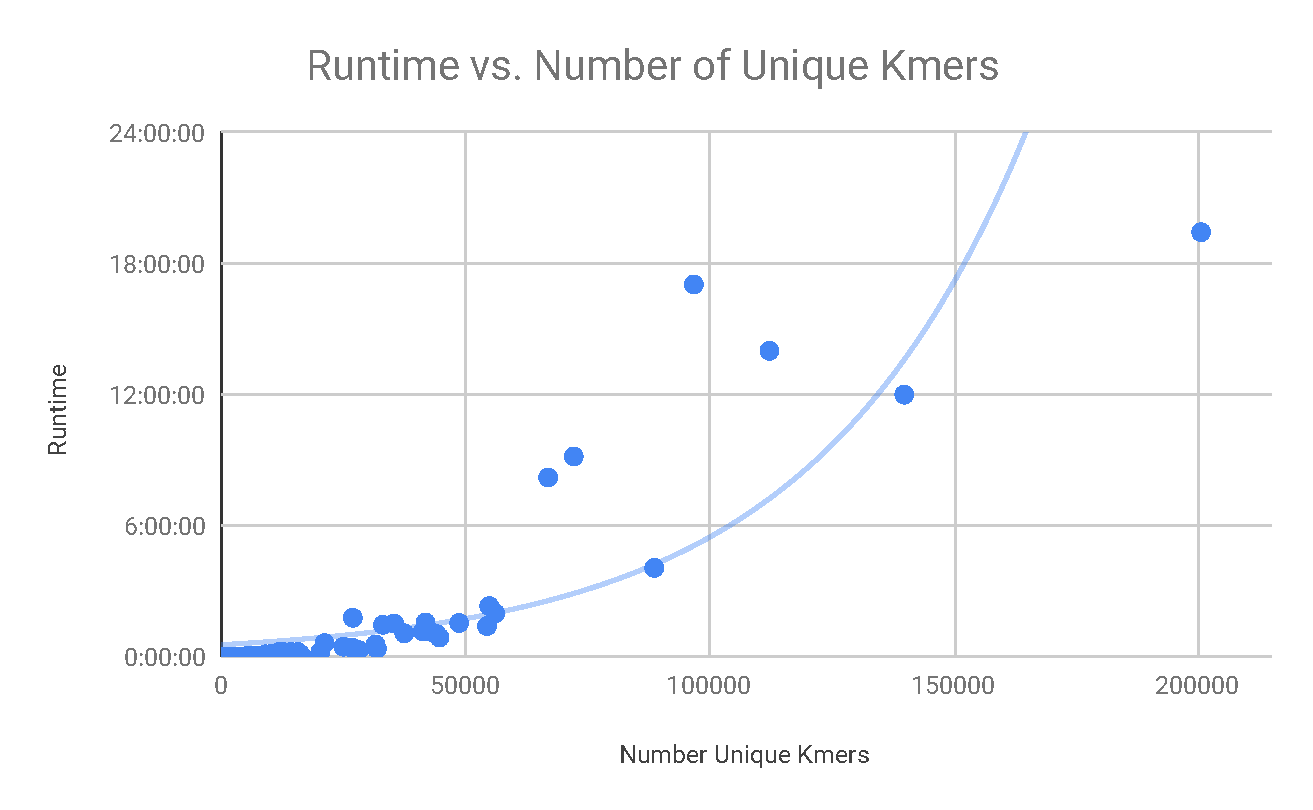
\includegraphics[width=0.5\colwidth]{figures/runtime.pdf}
      \caption{Runtime grows exponentially with respect to input size}
      \label{fig:runtime}
    \end{figure}
    \begin{figure}
      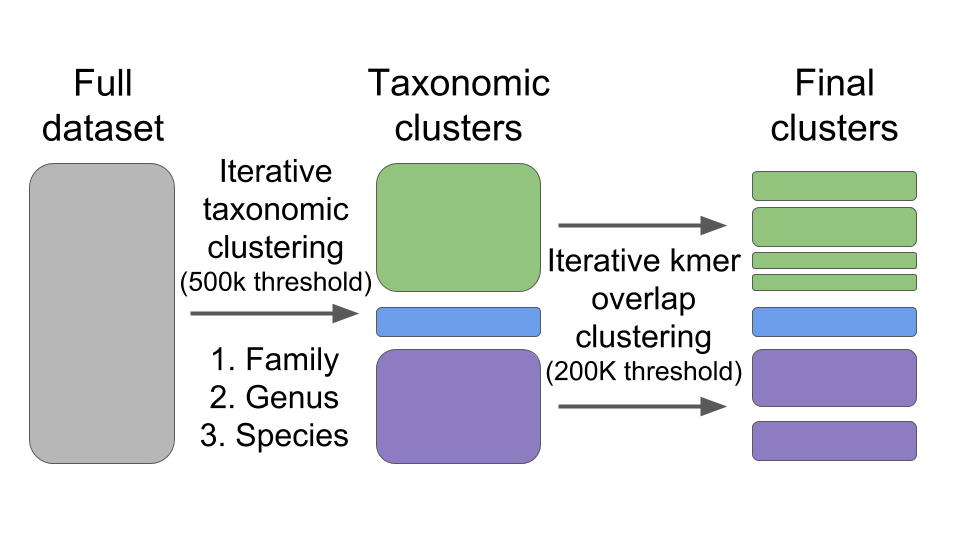
\includegraphics[width=0.5\colwidth]{figures/clustering.png}
      \caption{Visual Depiction of Clustering Process}
      \label{fig:clustering}
    \end{figure}
    \begin{itemize}
    \item Input data of $>1,000,000$ viral proteins is too large to run all at once in a reasonable amount of time,
      so clustering is used to break data down into more manageable pieces.
    \item Two Stages of clustering: 
      \begin{itemize}
      \item Taxonomic-Based: Few oligos shared between families,
        clustering by family doesn't result in loss of sensitivity
      \item Kmer-Based: Clustering by kmers creates clusters of similar sequences,
        good for our approach.
      \end{itemize}
    \end{itemize}

  \end{block}

  \begin{block}{Fusce aliquam magna velit}

    Et rutrum ex euismod vel. Pellentesque ultricies, velit in fermentum
    vestibulum, lectus nisi pretium nibh, sit amet aliquam lectus augue vel
    velit. Suspendisse rhoncus massa porttitor augue feugiat molestie. Sed
    molestie ut orci nec malesuada. Sed ultricies feugiat est fringilla
    posuere.

    \begin{figure}
      \centering
      \begin{tikzpicture}
        \begin{axis}[
            scale only axis,
            no markers,
            domain=0:2*pi,
            samples=100,
            axis lines=center,
            axis line style={-},
            ticks=none]
          \addplot[red] {sin(deg(x))};
          \addplot[blue] {cos(deg(x))};
        \end{axis}
      \end{tikzpicture}
      \caption{Another figure caption.}
    \end{figure}

  \end{block}

  \begin{block}{Nam cursus consequat egestas}

    Nulla eget sem quam. Ut aliquam volutpat nisi vestibulum convallis. Nunc a
    lectus et eros facilisis hendrerit eu non urna. Interdum et malesuada fames
    ac ante \textit{ipsum primis} in faucibus. Etiam sit amet velit eget sem
    euismod tristique. Praesent enim erat, porta vel mattis sed, pharetra sed
    ipsum. Morbi commodo condimentum massa, \textit{tempus venenatis} massa
    hendrerit quis. Maecenas sed porta est. Praesent mollis interdum lectus,
    sit amet sollicitudin risus tincidunt non.

    Etiam sit amet tempus lorem, aliquet condimentum velit. Donec et nibh
    consequat, sagittis ex eget, dictum orci. Etiam quis semper ante. Ut eu
    mauris purus. Proin nec consectetur ligula. Mauris pretium molestie
    ullamcorper. Integer nisi neque, aliquet et odio non, sagittis porta justo.

    \begin{itemize}
      \item \textbf{Sed consequat} id ante vel efficitur. Praesent congue massa
        sed est scelerisque, elementum mollis augue iaculis.
        \begin{itemize}
          \item In sed est finibus, vulputate
            nunc gravida, pulvinar lorem. In maximus nunc dolor, sed auctor eros
            porttitor quis.
          \item Fusce ornare dignissim nisi. Nam sit amet risus vel lacus
            tempor tincidunt eu a arcu.
          \item Donec rhoncus vestibulum erat, quis aliquam leo
            gravida egestas.
        \end{itemize}
      \item \textbf{Sed luctus, elit sit amet} dictum maximus, diam dolor
        faucibus purus, sed lobortis justo erat id turpis.
      \item \textbf{Pellentesque facilisis dolor in leo} bibendum congue.
        Maecenas congue finibus justo, vitae eleifend urna facilisis at.
    \end{itemize}

  \end{block}

\end{column}

\separatorcolumn

\begin{column}{\colwidth}

  \begin{block}{A block containing some math}

    Nullam non est elit. In eu ornare justo. Maecenas porttitor sodales lacus,
    ut cursus augue sodales ac.

    $$
    \int_{-\infty}^{\infty} e^{-x^2}\,dx = \sqrt{\pi}
    $$

    Interdum et malesuada fames $\{1, 4, 9, \ldots\}$ ac ante ipsum primis in
    faucibus. Cras eleifend dolor eu nulla suscipit suscipit. Sed lobortis non
    felis id vulputate.

    \heading{A heading inside a block}

    Praesent consectetur mi $x^2 + y^2$ metus, nec vestibulum justo viverra
    nec. Proin eget nulla pretium, egestas magna aliquam, mollis neque. Vivamus
    dictum $\mathbf{u}^\intercal\mathbf{v}$ sagittis odio, vel porta erat
    congue sed. Maecenas ut dolor quis arcu auctor porttitor.

    \heading{Another heading inside a block}

    Sed augue erat, scelerisque a purus ultricies, placerat porttitor neque.
    Donec $P(y \mid x)$ fermentum consectetur $\nabla_x P(y \mid x)$ sapien
    sagittis egestas. Duis eget leo euismod nunc viverra imperdiet nec id
    justo.

  \end{block}

  \begin{block}{Nullam vel erat at velit convallis laoreet}

    Class aptent taciti sociosqu ad litora torquent per conubia nostra, per
    inceptos himenaeos. Phasellus libero enim, gravida sed erat sit amet,
    scelerisque congue diam. Fusce dapibus dui ut augue pulvinar iaculis.

    \begin{table}
      \centering
      \begin{tabular}{l r r c}
        \toprule
        \textbf{First column} & \textbf{Second column} & \textbf{Third column} & \textbf{Fourth} \\
        \midrule
        Foo & 13.37 & 384,394 & $\alpha$ \\
        Bar & 2.17 & 1,392 & $\beta$ \\
        Baz & 3.14 & 83,742 & $\delta$ \\
        Qux & 7.59 & 974 & $\gamma$ \\
        \bottomrule
      \end{tabular}
      \caption{A table caption.}
    \end{table}

    Donec quis posuere ligula. Nunc feugiat elit a mi malesuada consequat. Sed
    imperdiet augue ac nibh aliquet tristique. Aenean eu tortor vulputate,
    eleifend lorem in, dictum urna. Proin auctor ante in augue tincidunt
    tempor. Proin pellentesque vulputate odio, ac gravida nulla posuere
    efficitur. Aenean at velit vel dolor blandit molestie. Mauris laoreet
    commodo quam, non luctus nibh ullamcorper in. Class aptent taciti sociosqu
    ad litora torquent per conubia nostra, per inceptos himenaeos.

    Nulla varius finibus volutpat. Mauris molestie lorem tincidunt, iaculis
    libero at, gravida ante. Phasellus at felis eu neque suscipit suscipit.
    Integer ullamcorper, dui nec pretium ornare, urna dolor consequat libero,
    in feugiat elit lorem euismod lacus. Pellentesque sit amet dolor mollis,
    auctor urna non, tempus sem.

  \end{block}

  \begin{block}{References}

    \nocite{*}
    \footnotesize{\bibliographystyle{plain}\bibliography{poster}}

  \end{block}

\end{column}

\separatorcolumn
\end{columns}
\end{frame}

\end{document}
